\documentclass{standalone}
\usepackage{tikz}
\usetikzlibrary{patterns, positioning}


\begin{document}
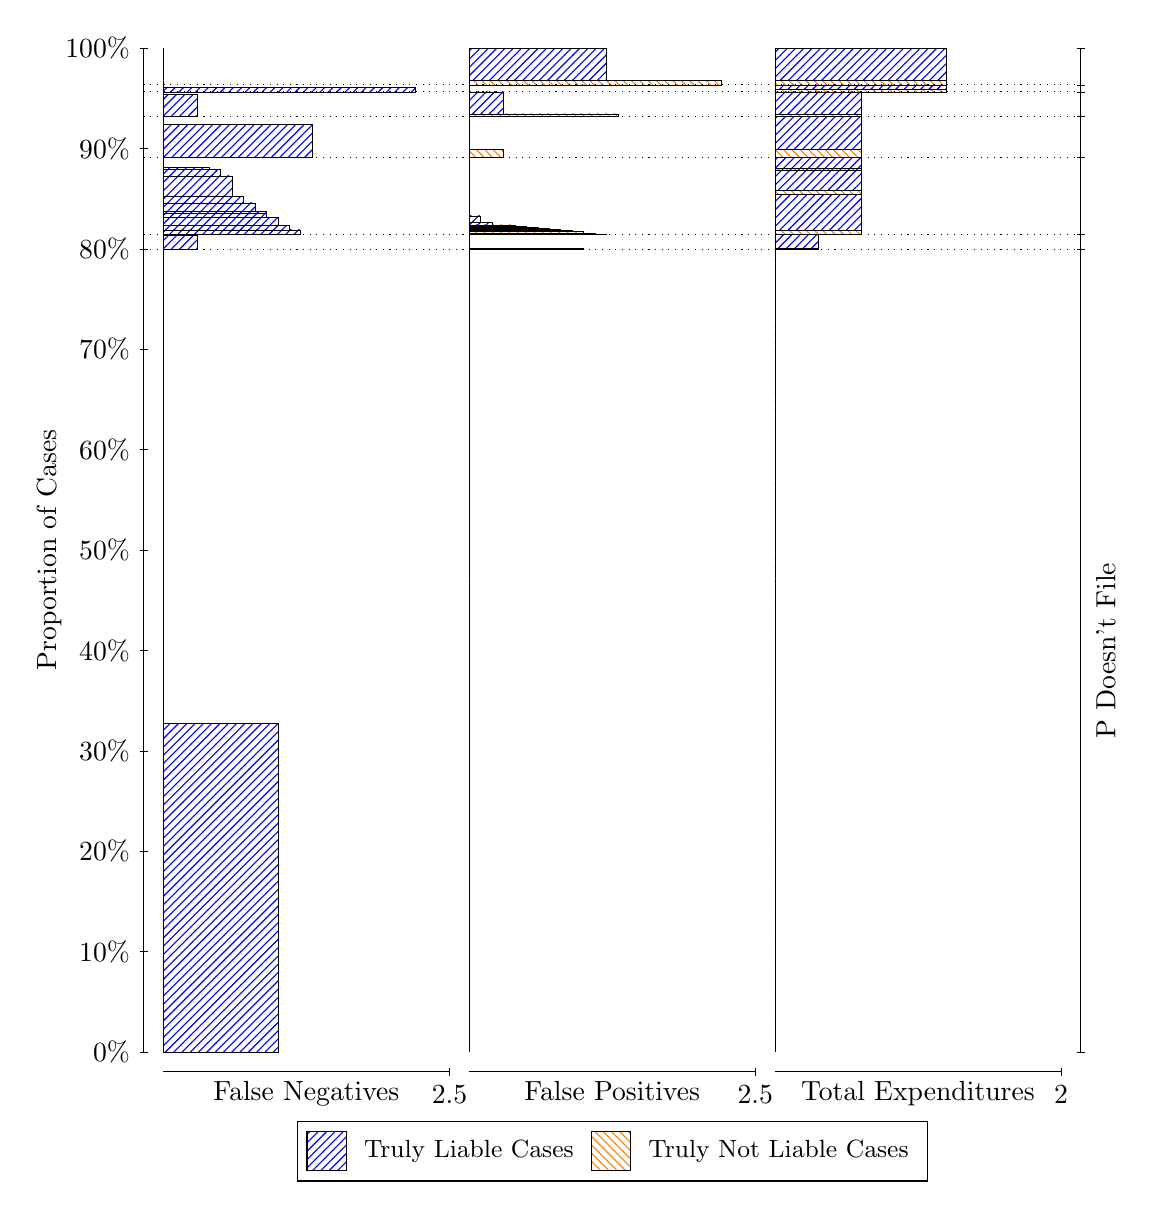
\begin{tikzpicture}
\draw[black, very thin] (1.5,1.75) -- (1.5,14.5);
\node[rotate=90, text=black, anchor=center] at (0.3, 8.125) {Proportion of Cases};
\draw[black, very thin] (1.45,1.75) -- (1.55,1.75);
\node[text=black, anchor=east] at (1.45, 1.75) {0\%};
\draw[black, very thin] (1.45,3.025) -- (1.55,3.025);
\node[text=black, anchor=east] at (1.45, 3.025) {10\%};
\draw[black, very thin] (1.45,4.3) -- (1.55,4.3);
\node[text=black, anchor=east] at (1.45, 4.3) {20\%};
\draw[black, very thin] (1.45,5.575) -- (1.55,5.575);
\node[text=black, anchor=east] at (1.45, 5.575) {30\%};
\draw[black, very thin] (1.45,6.85) -- (1.55,6.85);
\node[text=black, anchor=east] at (1.45, 6.85) {40\%};
\draw[black, very thin] (1.45,8.125) -- (1.55,8.125);
\node[text=black, anchor=east] at (1.45, 8.125) {50\%};
\draw[black, very thin] (1.45,9.4) -- (1.55,9.4);
\node[text=black, anchor=east] at (1.45, 9.4) {60\%};
\draw[black, very thin] (1.45,10.675) -- (1.55,10.675);
\node[text=black, anchor=east] at (1.45, 10.675) {70\%};
\draw[black, very thin] (1.45,11.95) -- (1.55,11.95);
\node[text=black, anchor=east] at (1.45, 11.95) {80\%};
\draw[black, very thin] (1.45,13.225) -- (1.55,13.225);
\node[text=black, anchor=east] at (1.45, 13.225) {90\%};
\draw[black, very thin] (1.45,14.5) -- (1.55,14.5);
\node[text=black, anchor=east] at (1.45, 14.5) {100\%};

\draw[black, very thin] (13.4,1.75) -- (13.4,14.5);
\draw[black, very thin] (13.35,1.75) -- (13.45,1.75);
\node[anchor=west] at (13.35, 1.75) {};
\draw[black, very thin] (13.35,11.942) -- (13.45,11.942);
\node[anchor=west] at (13.35, 11.942) {};
\draw[black, very thin] (13.35,12.133) -- (13.45,12.133);
\node[anchor=west] at (13.35, 12.133) {};
\draw[black, very thin] (13.35,13.108) -- (13.45,13.108);
\node[anchor=west] at (13.35, 13.108) {};
\draw[black, very thin] (13.35,13.632) -- (13.45,13.632);
\node[anchor=west] at (13.35, 13.632) {};
\draw[black, very thin] (13.35,13.944) -- (13.45,13.944);
\node[anchor=west] at (13.35, 13.944) {};
\draw[black, very thin] (13.35,14.033) -- (13.45,14.033);
\node[anchor=west] at (13.35, 14.033) {};
\draw[black, very thin] (13.35,14.5) -- (13.45,14.5);
\node[anchor=west] at (13.35, 14.5) {};

\draw[black, very thin, pattern color=blue, pattern=north east lines] (1.75,1.75) rectangle (3.2033,5.9267);
\draw[black, very thin, pattern color=orange, pattern=north west lines] (1.75,5.9267) rectangle (1.75,11.942);
\draw[black, very thin, pattern color=blue, pattern=north east lines] (1.75,11.942) rectangle (2.186,12.119);
\draw[black, very thin, pattern color=orange, pattern=north west lines] (1.75,12.119) rectangle (1.75,12.133);
\draw[black, very thin, pattern color=blue, pattern=north east lines] (1.75,12.133) rectangle (3.494,12.19);
\draw[black, very thin, pattern color=blue, pattern=north east lines] (1.75,12.19) rectangle (3.3487,12.249);
\draw[black, very thin, pattern color=blue, pattern=north east lines] (1.75,12.249) rectangle (3.2033,12.348);
\draw[black, very thin, pattern color=blue, pattern=north east lines] (1.75,12.348) rectangle (3.058,12.397);
\draw[black, very thin, pattern color=blue, pattern=north east lines] (1.75,12.397) rectangle (3.058,12.427);
\draw[black, very thin, pattern color=blue, pattern=north east lines] (1.75,12.427) rectangle (2.9127,12.533);
\draw[black, very thin, pattern color=blue, pattern=north east lines] (1.75,12.533) rectangle (2.7673,12.611);
\draw[black, very thin, pattern color=blue, pattern=north east lines] (1.75,12.611) rectangle (2.622,12.875);
\draw[black, very thin, pattern color=blue, pattern=north east lines] (1.75,12.875) rectangle (2.4767,12.958);
\draw[black, very thin, pattern color=blue, pattern=north east lines] (1.75,12.958) rectangle (2.3313,12.987);
\draw[black, very thin, pattern color=orange, pattern=north west lines] (1.75,12.987) rectangle (1.75,13.108);
\draw[black, very thin, pattern color=blue, pattern=north east lines] (1.75,13.108) rectangle (3.6393,13.531);
\draw[black, very thin, pattern color=orange, pattern=north west lines] (1.75,13.531) rectangle (1.75,13.632);
\draw[black, very thin, pattern color=blue, pattern=north east lines] (1.75,13.632) rectangle (2.186,13.912);
\draw[black, very thin, pattern color=orange, pattern=north west lines] (1.75,13.912) rectangle (1.75,13.944);
\draw[black, very thin, pattern color=blue, pattern=north east lines] (1.75,13.944) rectangle (4.9473,13.997);
\draw[black, very thin, pattern color=orange, pattern=north west lines] (1.75,13.997) rectangle (1.75,14.033);
\draw[black, very thin, pattern color=orange, pattern=north west lines] (1.75,14.033) rectangle (1.75,14.088);
\draw[black, very thin, pattern color=blue, pattern=north east lines] (1.75,14.088) rectangle (1.75,14.5);
\draw[black, very thin, pattern color=orange, pattern=north west lines] (5.6333,1.75) rectangle (5.6333,7.765);
\draw[black, very thin, pattern color=blue, pattern=north east lines] (5.6333,7.765) rectangle (5.6333,11.942);
\draw[black, very thin, pattern color=orange, pattern=north west lines] (5.6333,11.942) rectangle (7.0867,11.956);
\draw[black, very thin, pattern color=blue, pattern=north east lines] (5.6333,11.956) rectangle (5.6333,12.133);
\draw[black, very thin, pattern color=orange, pattern=north west lines] (5.6333,12.133) rectangle (7.3773,12.137);
\draw[black, very thin, pattern color=orange, pattern=north west lines] (5.6333,12.137) rectangle (7.232,12.146);
\draw[black, very thin, pattern color=orange, pattern=north west lines] (5.6333,12.146) rectangle (7.0867,12.172);
\draw[black, very thin, pattern color=orange, pattern=north west lines] (5.6333,12.172) rectangle (6.9413,12.182);
\draw[black, very thin, pattern color=orange, pattern=north west lines] (5.6333,12.182) rectangle (6.796,12.197);
\draw[black, very thin, pattern color=orange, pattern=north west lines] (5.6333,12.197) rectangle (6.6507,12.207);
\draw[black, very thin, pattern color=orange, pattern=north west lines] (5.6333,12.207) rectangle (6.5053,12.223);
\draw[black, very thin, pattern color=orange, pattern=north west lines] (5.6333,12.223) rectangle (6.36,12.232);
\draw[black, very thin, pattern color=orange, pattern=north west lines] (5.6333,12.232) rectangle (6.2147,12.255);
\draw[black, very thin, pattern color=blue, pattern=north east lines] (5.6333,12.255) rectangle (5.924,12.283);
\draw[black, very thin, pattern color=blue, pattern=north east lines] (5.6333,12.283) rectangle (5.7787,12.367);
\draw[black, very thin, pattern color=blue, pattern=north east lines] (5.6333,12.367) rectangle (5.6333,13.108);
\draw[black, very thin, pattern color=orange, pattern=north west lines] (5.6333,13.108) rectangle (6.0693,13.21);
\draw[black, very thin, pattern color=blue, pattern=north east lines] (5.6333,13.21) rectangle (5.6333,13.632);
\draw[black, very thin, pattern color=orange, pattern=north west lines] (5.6333,13.632) rectangle (7.5227,13.664);
\draw[black, very thin, pattern color=blue, pattern=north east lines] (5.6333,13.664) rectangle (6.0693,13.944);
\draw[black, very thin, pattern color=orange, pattern=north west lines] (5.6333,13.944) rectangle (5.6333,13.98);
\draw[black, very thin, pattern color=blue, pattern=north east lines] (5.6333,13.98) rectangle (5.6333,14.033);
\draw[black, very thin, pattern color=orange, pattern=north west lines] (5.6333,14.033) rectangle (8.8307,14.088);
\draw[black, very thin, pattern color=blue, pattern=north east lines] (5.6333,14.088) rectangle (7.3773,14.5);
\draw[black, very thin, pattern color=orange, pattern=north west lines] (9.5167,1.75) rectangle (9.5167,7.765);
\draw[black, very thin, pattern color=blue, pattern=north east lines] (9.5167,7.765) rectangle (9.5167,11.942);
\draw[black, very thin, pattern color=orange, pattern=north west lines] (9.5167,11.942) rectangle (10.062,11.956);
\draw[black, very thin, pattern color=blue, pattern=north east lines] (9.5167,11.956) rectangle (10.062,12.133);
\draw[black, very thin, pattern color=orange, pattern=north west lines] (9.5167,12.133) rectangle (10.607,12.183);
\draw[black, very thin, pattern color=blue, pattern=north east lines] (9.5167,12.183) rectangle (10.607,12.637);
\draw[black, very thin, pattern color=orange, pattern=north west lines] (9.5167,12.637) rectangle (10.607,12.69);
\draw[black, very thin, pattern color=blue, pattern=north east lines] (9.5167,12.69) rectangle (10.607,12.953);
\draw[black, very thin, pattern color=orange, pattern=north west lines] (9.5167,12.953) rectangle (10.607,12.972);
\draw[black, very thin, pattern color=blue, pattern=north east lines] (9.5167,12.972) rectangle (10.607,13.108);
\draw[black, very thin, pattern color=orange, pattern=north west lines] (9.5167,13.108) rectangle (10.607,13.21);
\draw[black, very thin, pattern color=blue, pattern=north east lines] (9.5167,13.21) rectangle (10.607,13.632);
\draw[black, very thin, pattern color=orange, pattern=north west lines] (9.5167,13.632) rectangle (10.607,13.664);
\draw[black, very thin, pattern color=blue, pattern=north east lines] (9.5167,13.664) rectangle (10.607,13.944);
\draw[black, very thin, pattern color=orange, pattern=north west lines] (9.5167,13.944) rectangle (11.697,13.98);
\draw[black, very thin, pattern color=blue, pattern=north east lines] (9.5167,13.98) rectangle (11.697,14.033);
\draw[black, very thin, pattern color=orange, pattern=north west lines] (9.5167,14.033) rectangle (11.697,14.088);
\draw[black, very thin, pattern color=blue, pattern=north east lines] (9.5167,14.088) rectangle (11.697,14.5);
\draw[black, dotted] (1.5,11.942) -- (13.4,11.942);
\draw[black, dotted] (1.5,12.133) -- (13.4,12.133);
\draw[black, dotted] (1.5,13.108) -- (13.4,13.108);
\draw[black, dotted] (1.5,13.632) -- (13.4,13.632);
\draw[black, dotted] (1.5,13.944) -- (13.4,13.944);
\draw[black, dotted] (1.5,14.033) -- (13.4,14.033);
\draw[black, very thin] (1.75,1.5) -- (5.3833,1.5);
\node[text=black, anchor=north] at (3.5667, 1.5) {False Negatives};
\draw[black, very thin] (5.3833,1.45) -- (5.3833,1.55);
\node[text=black, anchor=north] at (5.3833, 1.45) {2.5};

\draw[black, very thin] (5.6333,1.5) -- (9.2667,1.5);
\node[text=black, anchor=north] at (7.45, 1.5) {False Positives};
\draw[black, very thin] (9.2667,1.45) -- (9.2667,1.55);
\node[text=black, anchor=north] at (9.2667, 1.45) {2.5};

\draw[black, very thin] (9.5167,1.5) -- (13.15,1.5);
\node[text=black, anchor=north] at (11.333, 1.5) {Total Expenditures};
\draw[black, very thin] (13.15,1.45) -- (13.15,1.55);
\node[text=black, anchor=north] at (13.15, 1.45) {2};

\node[text=black, centered, rotate=90] at (13.72, 6.8458) {P Doesn't File};







\draw (7.449999999999999,1.5) node[draw=none] (baseCoordinate) {};
\begin{scope}[align=center]
        \matrix[scale=0.5, draw=black, below=0.5cm of baseCoordinate, nodes={draw}, column sep=0.1cm]{
            \node[rectangle, draw, minimum width=0.5cm, minimum height=0.5cm, pattern color=blue, pattern=north east lines] {}; &
            \node[draw=none, font=\small, text=black] (B) {Truly Liable Cases}; &
            \node[rectangle, draw, minimum width=0.5cm, minimum height=0.5cm, pattern color=orange, pattern=north west lines] {}; &
            \node[draw=none, font=\small, text=black] (B) {Truly Not Liable Cases}; \\
            };
\end{scope}

\end{tikzpicture}
\end{document}